\subsubsection{UC1 - Caricamento del dataset}
\begin{figure}[h]
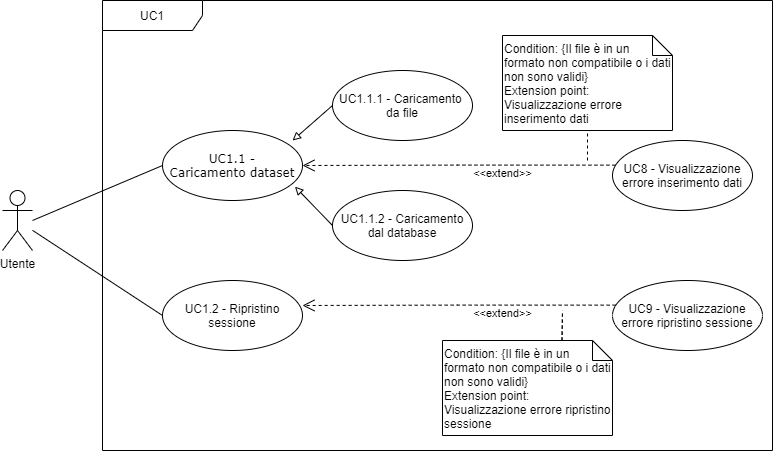
\includegraphics[width=\linewidth]{section/Images/UC1.png}
\centering
\caption{UC1 - Caricamento del dataset}
\end{figure}
\begin{itemize}
	\item \textbf{Attore primario}: Utente.
	\item \textbf{Precondizioni}: Il sistema è raggiungibile e funzionante.
	\item \textbf{Postcondizioni}: Viene visualizzato un messaggio che avvisa l'utente del corretto caricamento dei dati e della loro validità.
	\item \textbf{Scenario principale}:
		\begin{enumerate}
			\item L'utente accede al sistema;
			\item L'utente sceglie come importare i dati nel sistema:
				\begin{enumerate}[(a)]
			\item L'utente seleziona la funzionalità "carica file" [UC1.1];
			\item L'utente seleziona un dataset tra quelli disponibili nel database [UC1.2].
				\end{enumerate}
		\end{enumerate}
	\item \textbf{Estensioni}:
	\begin{enumerate}[(a)]
		\item Nel caso in cui il file sia in un formato sbagliato o i dati non sono validi:
		\begin{enumerate}[1.]
			\item I dati non vengono caricati nel sistema;
			\item Viene visualizzato un errore esplicativo [UCX].
		\end{enumerate}
	\end{enumerate}
\end{itemize}






  